\documentclass{article}
\usepackage[utf8]{inputenc}
%%\documentclass{article}
\usepackage{movie15}
\usepackage{graphicx}
\usepackage{amsmath}
\usepackage{amssymb}

\title{security_ARP Attack design}
%%\author{ }
\date{July 2019}


\vspace{1cm}
\hspace{5cm}
 
 \begin{center}
    \huge
    \textbf{ARP Cache Poisoning } 
    \\ \\ \\
 \end{center}
 
 
\begin{figure}[h]
    \centering

\includegraphics[width=0.2\textwidth]{images/buet_logo_1.png}

\end{figure}
 
 



\begin{center}
    \\
    \large
 Prepared By\\
MD.Omer Danish\\ \\
Student ID: 1505053
\\
Group No : 01\\
Section : A\\


\end{center}


\begin{center}
\large
Submitted to \\
Dr. Md. Shohrab Hossain\\
Associate Professor\\ \\
\newline \\
\Large
\\
Department of Computer Science \\ \\
Bangladesh University of Engineering and Technology\\ \\ \\
\linebreak

\end{center}


\date{\today}



\newpage




\begin{document}
\tableofcontents
\newpage
%%\maketitle

\section{Introduction to ARP Cache Poisoning}
\textbf{ARP Cache Poisoning} is a technique by which an attacker sends (spoofed) Address Resolution Protocol (ARP) messages onto a local area network. Generally, the aim is to associate the attacker's MAC address with the IP address of another host, such as the default gateway, causing any traffic meant for that IP address to be sent to the attacker instead.

\begin{figure}[h]
    \centering
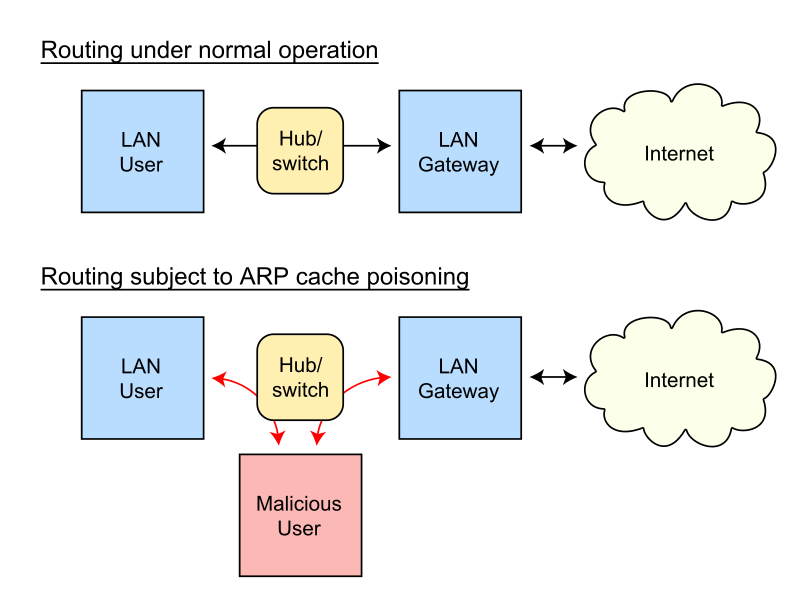
\includegraphics[width=\textwidth]{images/arp.jpg}
\captioig  ARP poisoning attack
\end{figure}

\section{Effect of ARP Cache Poisoning}
\textbf{ARP Cache Poisoning} can create many unusual behavior in  network. Some of them are 
\renewcommand\labelitemi{$\square$}
\begin{itemize}
    \item  Denial of service
    \item  Man in the middle,
    \item  Session hijacking
    \item Stop all traffic
    
\end{itemize}


\section{How ARP Works??}
The Address Resolution Protocol (ARP) is used communications protocol for resolving Internet layer addresses into link layer addresses.

When an Internet Protocol (IP) datagram is sent from one host to another in a local area network, the destination IP address must be resolved to a MAC address for transmission via the data link layer. When another host's IP address is known, and its MAC address is needed, a broadcast packet is sent out on the local network. This packet is known as an ARP request. The destination machine with the IP in the ARP request then responds with an ARP reply that contains the MAC address for that IP.

\section{ARP vulnerabilities}
ARP is a stateless protocol. Network hosts will automatically cache any ARP replies they receive, regardless of whether network hosts requested them. Even ARP entries that have not yet expired will be overwritten when a new ARP reply packet is received. There is no method in the ARP protocol by which a host can authenticate the peer from which the packet originated. This behavior is the vulnerability that allows ARP spoofing to occur.

\section{How ARP Cache Poisoning Works}

The basic principle behind ARP spoofing is to exploit the lack of authentication in the ARP protocol by sending spoofed ARP messages onto the LAN.ARP spoofing attacks can be run  from an attacker's machine that is connected directly to the target LAN.

\par  The goal of the attack is to associate the attacker's host MAC address with the IP address of a target host, so that any traffic meant for the target host will be sent to the attacker's host.


\par The attacker may choose to do three tasks 
 
\begin{enumerate}
\item  Launch a denial-of-service attack
\item  Inspect the packets (spying)
\item Modify the data before forwarding it (man-in-the-middle attack)
\end{enumerate}


\section{ARP Request and Reply Message }

The purpose of Address Resolution Protocol (ARP) is to find out the MAC address of a device in your Local Area Network (LAN), for the corresponding IPv4 address, which network application is trying to communicate.

\begin{figure}[h]
    \centering
%%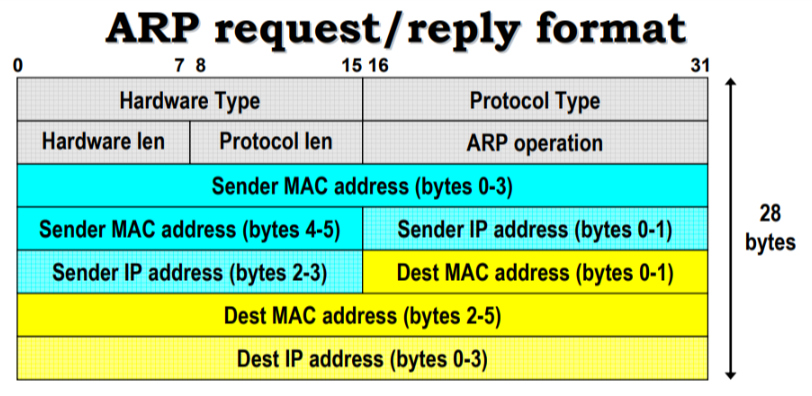
\includegraphics[width=\textwidth]{images/arp_req_reply.png}
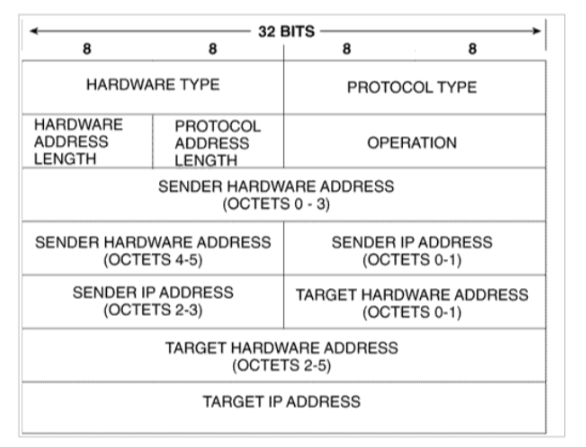
\includegraphics[width=\textwidth]{images/arp_2.png}
\captioig ARP message format 
\end{figure}

Following are the fields in the Address Resolution Protocol (ARP) Message Format.
\par\newline
\textbf{Hardware Type: } It specifies the type of hardware used for the local network transmitting the ARP message. 
\par\newline
\textbf{Protocol Type:} Each protocol is assigned a number used in this field. 
\par\newline
\textbf{Hardware Address Length:}This is the length in bytes of a hardware (MAC) address.
\par\newline
\textbf{Protocol Address Length:} Length in bytes of a logical address (IPv4 Address). IPv4 addresses are 4 bytes long.
\par\newline
\textbf{Opcode:} It the nature of the ARP message. 1 for ARP request and 2 for ARP reply.
\par\newline
\textbf{Sender Hardware Address:} MAC Address  address of the device sending the message.
\par\newline
\textbf{Sender Protocol Address:} IP  of the device sending the message
\par\newline
\textbf{Target Hardware Address:} MAC Address of the intended receiver. This field is ignored in requests.
\par\newline
\textbf{Target Protocol Address:} IP of the intended receiver.


\begin{figure}[bp!]
\centering
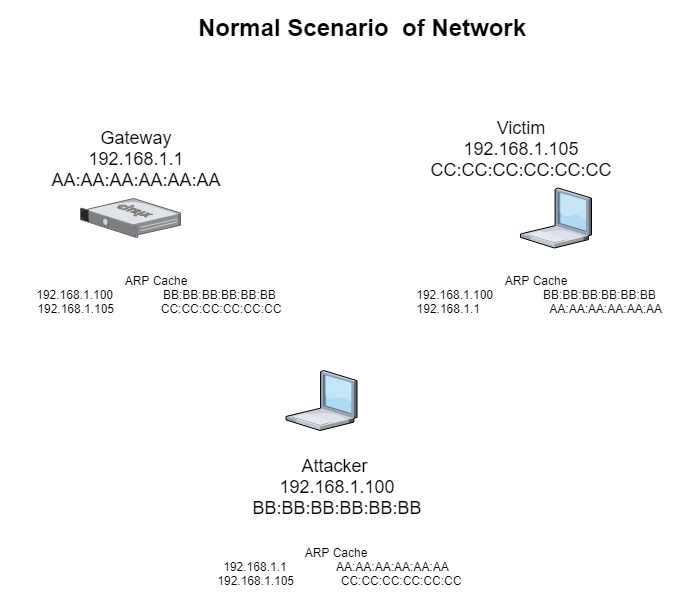
\includegraphics[width=\textwidth,scale=0.8]{images/Normal_Scenario_of_Diagram.png}
\captioig Normal Scenario 
\end{figure}
\newpage
\begin{figure}[hbp!]
\centering
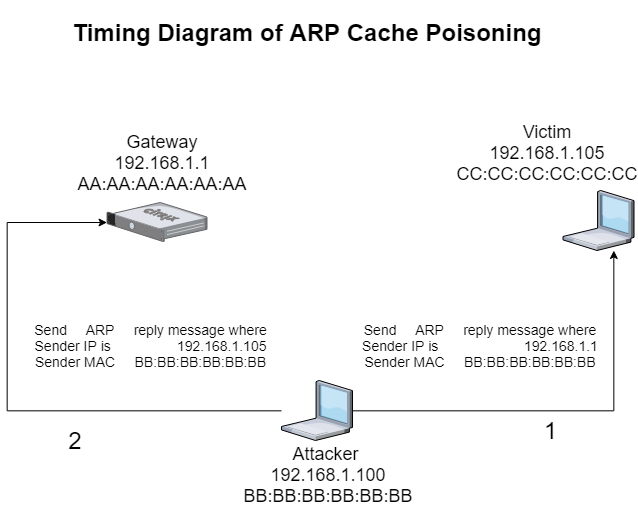
\includegraphics[width=\textwidth,height=14cm]{images/ARP_Cache_Poisoning_Timing_Diagram.png}
\captioig Timing Diagram of Attack
\end{figure}


\begin{figure}[bp!]
\centering
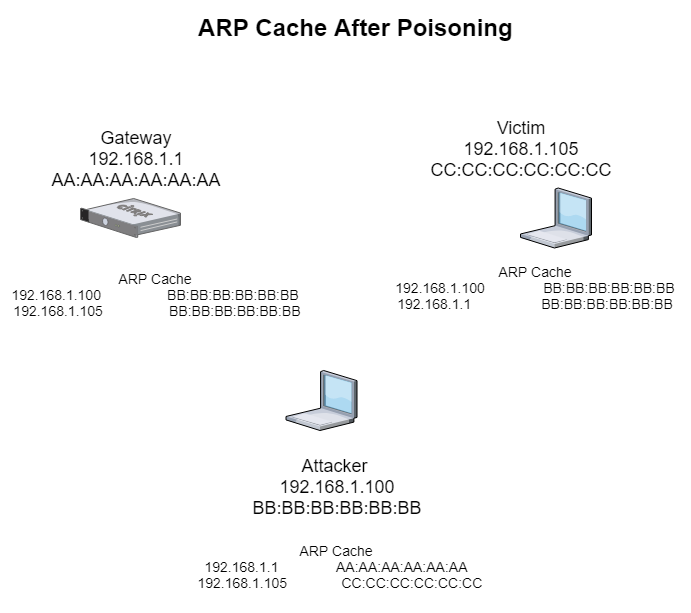
\includegraphics[width=\textwidth,height=16cm]{images/ARP_Cache_After_Poisoning.png}
\captioig ARP Cache after Attack 
\end{figure}


\section{How The Attack Works}

Sending malicious ARP packets to a default gateway on a LAN in order to change the pairings in its IP to MAC address table. ARP Protocol translates IP addresses into MAC addresses.  ARP Poisoning attacks are extremely easy to carry out as long as the attacker has control of a machine within the target LAN or is directly connected to it.

The attack itself consists of an attacker sending a false ARP reply message to the default network gateway, informing it that attacker's (here it is me ) MAC address should be associated with my target's IP address (and vice-versa, so my victim's  MAC is now associated with the attacker's (my) IP address).
%%Once the default gateway has received this message and broadcasts its changes to all other devices on the network, all of the target's traffic to any other device on the network travels through the attacker's computer, allowing the attacker to inspect or modify it before forwarding it to its real destination.
%%
Because ARP Poisoning attacks occur on such a low level, users targeted by ARP Poisoning rarely realize that their traffic is being inspected or modified. Besides Man-in-the-Middle Attacks, ARP Poisoning can be used to cause a denial-of-service condition over a LAN by simply intercepting or dropping and not forwarding the target's packets.


 
\section{Why It Should  Work}

ARP is a stateless protocol.Because the ARP protocol was designed purely for efficiency and not for security. 
\renewcommand\labelitemi{$\square$}
\begin{itemize}
    \item 
Network hosts will automatically cache any ARP replies they receive, regardless of whether network hosts requested them. Even ARP entries that have not yet expired will be overwritten when a new ARP reply packet is received.
    \item There is no method in the ARP protocol by which a host can authenticate the peer from which the packet originated. This behavior is the vulnerability that allows ARP Cache Poisoning to occur.
    
\end{itemize}


\end{document}
